\documentclass[tikz]{standalone}
\begin{document}
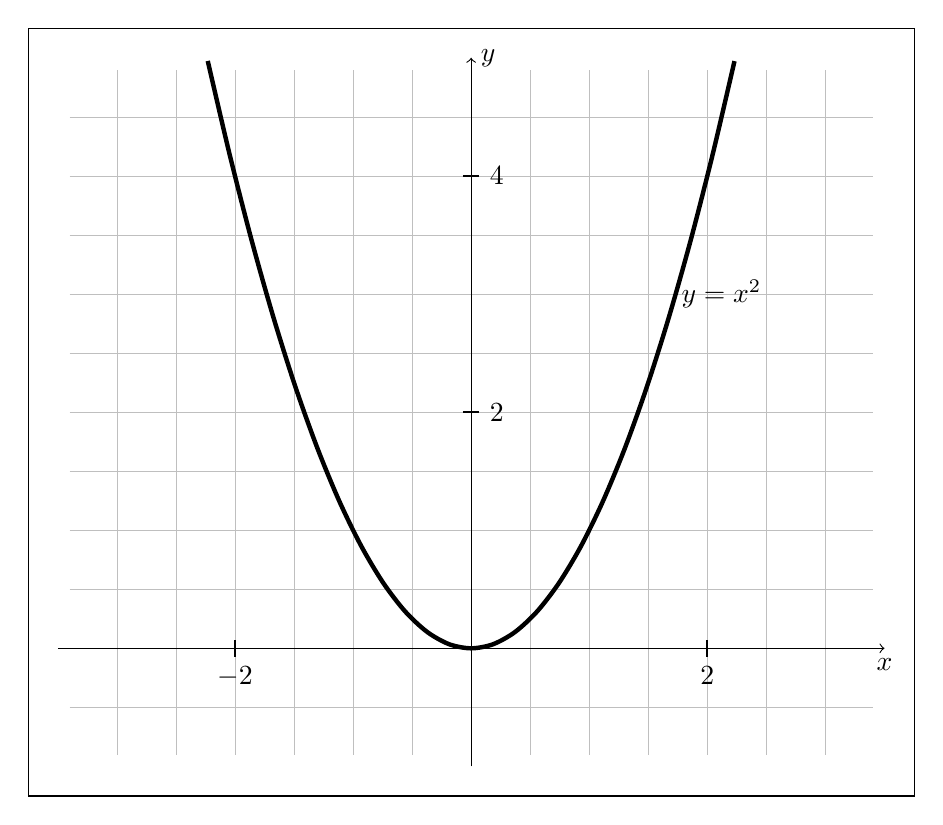
\begin{tikzpicture}[scale=1.5]

\draw[black,fill=white] (-3.75,-1.25) rectangle (3.75,5.25);
\draw[very thin,color=lightgray,step=0.5] (-3.4,-0.9) grid (3.4,4.9);
%\draw[very thin,color=gray,step=2] (-3.5,-1) grid (3.5,5);

\draw[->] (-3.5,0) -- (3.5,0) node[below] {$x$};
\draw[->] (0,-1) -- (0,5) node[right] {$y$};
\draw[domain=-2.23:2.23,smooth,variable=\x,black,ultra thick] plot ({\x},{\x*\x});%  node[right] {$y=x^2$};
       
\node[right] at (1.7, 3){$y = x^2$};

% tick marks
\foreach \x in {-2,2} 
	\draw [thick] (\x cm,2pt) -- (\x cm,-2pt) node[below] {$\x$};
\foreach \y in {2,4} 
	\draw [thick] (-2pt,\y cm) -- (2pt,\y cm) node[right] {$\y$};
\end{tikzpicture}
\end{document}
